 \documentclass[book.tex]{subfiles}
\begin{document}

\section{Performance and other Tricks}
Various smart techniques were employed to ensure every CPU cycle counted. This section explores some of the techniques used in Commander Keen.

\subsection{Tile caching}
When updating the master screen in VRAM, the engine copies each tile from RAM to VRAM. Each pixel requires a read and write operation to the four memory banks. As explained in section \ref{section:optimize_tile}, by reprogramming the latches on the EGA card, it was possible to copy four bytes at once from one VRAM location to another VRAM location. This trick could be applied to tiles if they contained only a background tile with no foreground layer.\\

\par
Once a background tile is loaded into the master screen, any subsequent requests for the same tile can be handled by copying it directly from VRAM, applying the reprogrammed latches, rather than from RAM to VRAM. The engine only needs to maintain which background tiles are already loaded into VRAM, which is done via an array.\\

\par
\begin{minipage}{\textwidth}
  \lstinputlisting[language=C]{code/tile_cache.c}
\end{minipage}
\par

The assembly function \cw{RFL\_NewTile} is responsible for drawing tiles to the master screen. It first checks if the background tile is already available in the tile cache array. If it is, the tile is copied with 32 bits per cycle from VRAM. If it is not, the tile is loaded from RAM, and the memory pointer in VRAM for that tile is stored in the tile cache array, allowing future requests to be served from VRAM.\\

\par
\begin{minipage}{\textwidth}
  \lstinputlisting[language={[x86masm]Assembler}]{code/RFL_NewTile.ASM}
\end{minipage}
\par

\subsection{Memory alignment}
The 286 CPU can read and write 16 bits in a single cycle, but there is a caveat: this only works when accessing even memory addresses. Even worse, writing a word at offset address \cw{FFFFh} causes an exception. \\

\par
Since a tile is word-aligned (16 bits wide) and the screen is refreshed in tile-size steps, it is always aligned with even memory addresses. However, this is not the case for sprites, which are byte-aligned. When a sprite is drawn starting from an odd memory address, the CPU can only read and write 8 bits at a time. To utilize the 16-bit data bus and avoiding the memory exception,  the engine first checks whether the destination is at an even or odd memory address. If the address is odd, it first writes a byte to VRAM to align the next operation to an even address, after which it continues writing in 16-bit words. To optimize sprite writing to VRAM, the engine uses small function routines for each combination of sprite width and even/odd address alignment.\\

\begin{figure}[H]
\centering
\begin{table}[H]
\begin{tabularx}{\textwidth}[c]{|X|X|X|}
\hline
  & \multicolumn{2}{c|}{\textbf{Start address}} \\ \hline
\textbf{Sprite width (bytes)} & \textbf{Even} & \textbf{Odd} \\ \hline
1 & Byte & Byte \\ \hline
2 & Word & Byte, Byte \\ \hline 
3 & Word, Byte & Byte, Word \\ \hline
4 & Word, Word & Byte, Word, Byte \\ \hline
5 & Word, Word, Byte & Byte, Word, Word \\ \hline
6 & Word, Word, Word & Byte, Word, Word, Byte \\ \hline
7 & Word, Word, Word, Byte & Byte, Word, Word, Word \\ \hline
8 & Word, Word, Word, Word & Byte, Word, Word, Word, Byte \\ \hline
9 & Word, Word, Word, Word, Byte & Byte, Word, Word, Word, Word \\ \hline
10 & Word, Word, Word, Word, Word & Byte, Word, Word, Word, Word, Byte \\ \hline

\end{tabularx}
\end{table}
\end{figure}

\par
\begin{minipage}{\textwidth}
  \lstinputlisting[language={[x86masm]Assembler}]{code/mask_routines.asm}
\end{minipage}
\par

Each function pointer is stored in a \cw{maskroutines} array. By cleverly using bit-shift operations and the Carry Flag (CF), the engine calls the appropriate function to write the sprite to VRAM.

\par
\begin{minipage}{\textwidth}
  \lstinputlisting[language={[x86masm]Assembler}]{code/VW_MaskBlock.asm}
\end{minipage}
\par


\subsection{Bouncing Physics}
When Keen throws a flower it bounces of the walls. For flat walls and floors the bounce can be easily calculated by reversing either the x-speed (for vertical walls) or y-speed (for horizontal walls). It becomes more complicated for slopes. Making an accurate calculation of the bounce on a slope requires expensive \cw{cos} and \cw{sin} methods. \\
\par
Instead, the game used a simple algorithm that approximates the angle to either 22$^{\circ}$, 45$^{\circ}$, 67$^{\circ}$ or 90$^{\circ}$. Based on the ratio between the x- and y-speed it calculates the resulting speed and corresponding angle. \\
\par
\begin{figure}[H]
\centering
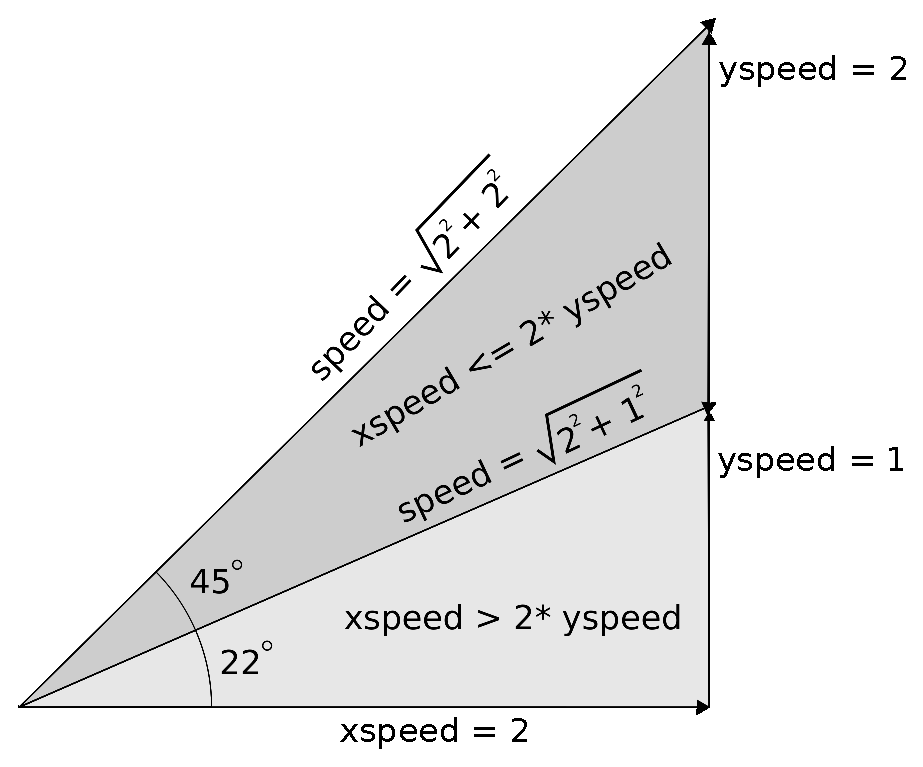
\includegraphics[width=0.8\textwidth]{imgs/drawings/angle_0.eps}
\label{fig:angles}
\end{figure}
\par

The speed is calculated as a factor of either the x- or y-speed, depending which of the two has the largest absolute value. Notice that for higher precision the speed is multiplied with 256.\\
\par
\begin{minipage}{\textwidth}
  \lstinputlisting[language=C]{code/calc_angle.c}
\end{minipage}
\par

For each combination of the eight type of slopes (Figure \ref{fig:walltype}) and incoming angle, the corresponding bounce angle is calculated using a simple lookup table.\\

\par
\begin{minipage}{\textwidth}
  \lstinputlisting[language=C]{code/bounceangle_lookup.c}
\end{minipage}
\par

The value in the table refers to the corresponding bounce angle calculation. As example, walltype 3 with incoming angle of 22$^{\circ}$, results in bounce calculation case 5.

\par
\begin{figure}[H]
\centering
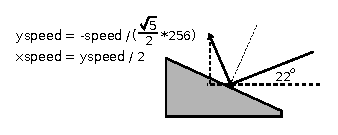
\includegraphics[width=0.7\textwidth]{imgs/drawings/bounce_angle.eps}
\caption{Walltype 3 with incoming angle of 22$^{\circ}$ (angle=0).}
\label{fig:bounce_angles}
\end{figure}
\par

\par
\begin{minipage}{\textwidth}
  \lstinputlisting[language=C]{code/angle.c}
\end{minipage}
\par

Notice that in several cases the bounce angle is not following the laws of physics. As example, for an incoming angle of 22$^{\circ}$ on a 45$^{\circ}$ slope the bounce angle is 90$^{\circ}$, instead of 67$^{\circ}$.
\par
\begin{figure}[H]
\centering
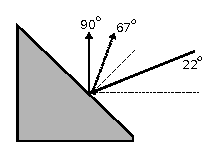
\includegraphics[width=0.4\textwidth]{imgs/drawings/bounce_physics.eps}
\end{figure}
\par

\pagebreak

\subsection{Pseudo Random Generator}
Random numbers are necessary for many things during runtime, such as calculating whether an enemy is able to hit the player based on its accuracy. This is achieved with a precalculated pseudo-random series of 256 elements.\\
\par
\begin{minipage}{\textwidth}
\lstinputlisting[language={[x86masm]Assembler}, style=mystyle,basicstyle=\small]{code/rndtable.asm}
\end{minipage}
\par
 Each entry in the array has a dual function. It is an integer within the range [0-255]\footnote{Or at least it was intended to!} and it is also the index of the next entry to fetch for next call. This works overall as a 255 entry chained list. The pseudo-random series is initialized using the current time modulo 256 when the engine starts up.\\

\par
\begin{minipage}{\textwidth}
\lstinputlisting[language={[x86masm]Assembler}]{code/US_InitRndT.asm}
\end{minipage}\\
\par
The random number generator saves the last index in \cw{rndindex}. Upon request for a new number, it simply looks up the new value and updates \cw{rndindex}.
\par
\begin{minipage}{\textwidth}
\lstinputlisting[ language={[x86masm]Assembler}]{code/US_RndT.asm}
\end{minipage}

\subsection{Screen fades}
When a new level is loaded, the screen fades from black to the default colors. Here it makes use of reassigning the color palette. This can easily be done by calling BIOS software interrupt \cw{10h}.\\


\par
\begin{minipage}{\textwidth}
  \lstinputlisting[language={[x86masm]Assembler}]{code/ega_set_palette.c}
\end{minipage}
\label{ega_set_palette}
\par

Earlier in the hardware chapter, Section \ref{sec:ega_color_palette}, it was explained that most EGA monitors did not support the extended 64-color rgbRGB palette, but kept the CGA pin assignment. That means applying "rgbRGB" results in wrong color mapping to the monitor. To better understand this, let's have a look at the pin signals.\\

\begin{figure}[H]
\centering
\begin{table}[H]
\begin{tabularx}{\textwidth}[c]{|>{\hsize=.16\hsize}X |>{\hsize=.42\hsize}X |>{\hsize=.42\hsize}X |}
\hline
\textbf{\color{black} Pin} & \textbf{\color{black} EGA modes (rgbRGB)} & \textbf{\color{black} CGA modes (RGBI)} \\
\hline
\color{black} 1 & \color{black} Ground &\color{black}Ground \\
\hline
\color{black} 2 & \color{white}\cellcolor{EGA_I_Red} Secondary Red (Intensity) &\color{black}Ground \\
\hline
\color{black} 3 & \color{white}\cellcolor{CGA_Red} Primary Red &\color{white}\cellcolor{CGA_Red} Red \\
\hline
\color{black} 4 & \color{black}\cellcolor{CGA_Green} Primary Green &\color{black}\cellcolor{CGA_Green} Green \\
\hline
\color{black} 5 & \color{white}\cellcolor{CGA_Blue} Primary Blue &\color{white}\cellcolor{CGA_Blue} Blue \\
\hline
\color{black} 6 & \color{black}\cellcolor{EGA_I_Green} Secondary Green (Intensity) &\color{white}\cellcolor{CGA_Dark_Grey}Intensity \\
\hline
\color{black} 7 & \color{white}\cellcolor{EGA_I_Blue} Secondary Blue (Intensity) &\color{black}Reserved \\
\hline
\color{black} 8 & \color{black} Horizontal Sync &\color{black}Horizontal Sync \\
\hline
\color{black} 9 & \color{black} Vertical Sync &\color{black}Vertical Sync \\

\hline

\end{tabularx}
\end{table}
\caption{EGA and CGA DE-9 connector pin signals.}
\label{pin_signals}
 \end{figure}
 
If one assigns the color brown (rgbRGB is \cw{010100b}) to one of the color indexes, the resulting color on the CGA pin assignment is light red; The secondary green pin ("r" in rgbRGB) is mapped to the Intensity pin in CGA mode, which results color red with intensity and not the expected brown color. So mapping the color to one of the indexes is based on "RGBI", using the Secondary Green ("r") for the  intensity. The "b" has no meaning and the "r" (Ground) is normally set to 0.\\

\par
By calling \cw{\_AX=1002h} the entire palette can be reprogrammed. In this case \cw{ES:BX} points to 17 bytes; an rgbRGB value for each of 16 palette index plus one for the border.
The screen fading is defined by the \cw{colors[7][17]} scheme. Note that the "b" bit is set for all intensity colors, but this had no effect on the results since the pin is unassigned for CGA.

\begin{figure}[H]
\centering
\setlength{\tabcolsep}{2pt} % set border margin to 3
\small
\begin{tabularx}{\textwidth}[c]{|+X|+X|+X|+X|+X|+X|+X|+X|+X|+X|+X|+X|+X|+X|+X|+X|+X|+X|}  
\hline

\rowcolor{CGA_White}\rowstyle{\color{black}}  \textbf{\#} & \textbf{0} & \textbf{1} & \textbf{2} & \textbf{3} & \textbf{4} & \textbf{5} & \textbf{6} & \textbf{7} & \textbf{8} & \textbf{9} & \textbf{10} & \textbf{11} & \textbf{12} & \textbf{13} & \textbf{14} & \textbf{15} & \textbf{16} \\ \hline

\rowcolor{CGA_Black}\rowstyle{\color{white}}   \cellcolor{CGA_White}\color{black} 0 &0& 0 & 0 & 0 & 0 & 0 & 0 & 0 & 0 & 0 & 0 & 0 & 0 & 0 & 0 & 0 & 0\\ \hline

\rowcolor{CGA_Black}\rowstyle{\color{white}}  \cellcolor{CGA_White}\color{black} 1 & 0 & 0 & 0 & 0 & 0 & 0 & 0 & 0 & 0 & \cellcolor{CGA_Blue} 1 & \cellcolor{CGA_Green}2 & \cellcolor{CGA_Cyan}3 & \cellcolor{CGA_Red}4 & \cellcolor{CGA_Magenta}5 & \cellcolor{CGA_Brown}6 & \cellcolor{CGA_Light_Grey}7  & 0\\ \hline

\rowcolor{CGA_Black}\rowstyle{\color{white}}  \cellcolor{CGA_White}\color{black} 2 & 0 & 0 & 0 & 0 & 0 & 0 & 0 & 0 & \cellcolor{CGA_Dark_Grey}0x18 & \cellcolor{CGA_Bright_Blue}0x19 & \cellcolor{CGA_Bright_Green}\color{black}0x1a & \cellcolor{CGA_Bright_Cyan}\color{black}0x1b & \cellcolor{CGA_Bright_Red}\color{black}0x1c & \cellcolor{CGA_Bright_Magenta}\color{black}0x1d & \cellcolor{CGA_Bright_Brown}\color{black}0x1e & \cellcolor{CGA_White}\color{black}0x1f & 0\\ \hline

\rowcolor{CGA_Black}\rowstyle{\color{white}}  \cellcolor{CGA_White}\color{black} 3 & 0 & \cellcolor{CGA_Blue} 1 & \cellcolor{CGA_Green}2 & \cellcolor{CGA_Cyan}3 & \cellcolor{CGA_Red}4 & \cellcolor{CGA_Magenta}5 & \cellcolor{CGA_Brown}6 & \cellcolor{CGA_Light_Grey}7 & \cellcolor{CGA_Dark_Grey}0x18 & \cellcolor{CGA_Bright_Blue}0x19 & \cellcolor{CGA_Bright_Green}\color{black}0x1a & \cellcolor{CGA_Bright_Cyan}\color{black}0x1b & \cellcolor{CGA_Bright_Red}\color{black}0x1c & \cellcolor{CGA_Bright_Magenta}\color{black}0x1d & \cellcolor{CGA_Bright_Brown}\color{black}0x1e & \cellcolor{CGA_White}\color{black}0x1f & 0\\ \hline

\rowcolor{CGA_White}\rowstyle{\color{white}}  \cellcolor{CGA_White}\color{black} 4 & \cellcolor{CGA_Black}0& \cellcolor{CGA_Blue} 1 & \cellcolor{CGA_Green}2 & \cellcolor{CGA_Cyan}3 & \cellcolor{CGA_Red}4 & \cellcolor{CGA_Magenta}5 & \cellcolor{CGA_Brown}6 & \cellcolor{CGA_Light_Grey}7 & \color{black}0x1f & \color{black}0x1f & \color{black}0x1f & \color{black}0x1f & \color{black}0x1f & \color{black}0x1f & \color{black}0x1f & \color{black}0x1f & \cellcolor{CGA_Black}0\\ \hline

\rowcolor{CGA_White}\rowstyle{\color{black}}  5&0x1f& 0x1f & 0x1f & 0x1f & 0x1f & 0x1f & 0x1f & 0x1f & 0x1f & 0x1f & 0x1f & 0x1f & 0x1f & 0x1f & 0x1f & 0x1f & 0x1f\\ \hline

\end{tabularx}\\
\setlength{\tabcolsep}{6pt} % reset border margin
\caption{Color fading table.}
\end{figure}

Fading in the screen from black to color is rather straight forward.\\
\par
\begin{minipage}{\textwidth}
  \lstinputlisting[language=C]{code/ega_fade_in.c}
\end{minipage}
\label{ega_fade_in}
\par


\end{document}



